\documentclass{beamer}

\usepackage{amsmath}
\usepackage{graphicx}
\usepackage{hyperref}
\usepackage{fontawesome5}
\usepackage{listings}
\usepackage{textcomp}

\graphicspath{{../img/}}

% Specify the theme
\usetheme{Madrid}

% Title and author information
\title{Recommender Systems Challenge 2023}
\author{Lorenzo Campana}

\institute{Politecnico di Milano}
\date{\today}

\begin{document}

% Title slide
\begin{frame}
  \titlepage\center Personal Code: 10605775
\end{frame}

% Content slides
\begin{frame}{Overview}
  \begin{itemize}
    \item $\approx 600k$ user-book interactions ($\approx 13k$ users, $\approx 22k$ books)
    \item Implicit ratings
    \item Provided slides results consider $80\%$ training, $20\%$ test
    \item Evaluation metric: MAP@10 
      \[
      \text{MAP@}K = \frac{1}{K} \sum_{u=1}^{N} \frac{1}{\min(K, m)} \sum_{k=1}^{K} P(k) * rel(k)
      \]
  \end{itemize}
\end{frame}

\begin{frame}{Baseline}
  \begin{block}{Top Popular algorithm}
    Identify the most frequently occurring books
  \end{block}
  \begin{itemize}
    \item Non Personalized
    \item $\text{MAP@}10=0.011742$
    \item How was it used?
    \begin{itemize}
      \item To provide recommendation to new users
    \end{itemize}
  \end{itemize}
\end{frame}

\begin{frame}{Hyperparameter tuning}
  \begin{itemize}
    \item Optuna
    \item 5 Folds Cross Validation
    \item $\text{\text{AWS free tier}} \approx $ \texteuro2.25
  \end{itemize}
  \begin{figure}
    \vspace{1cm}
    \centering
    
\includegraphics[width=0.5\textwidth]{diagram_aws_optuna_1.png}
    \caption{Optuna easy parallelization}
  \end{figure}
  
\end{frame}


\begin{frame}
  \frametitle{Directory tree structure}
  \begin{figure}
      \centering
      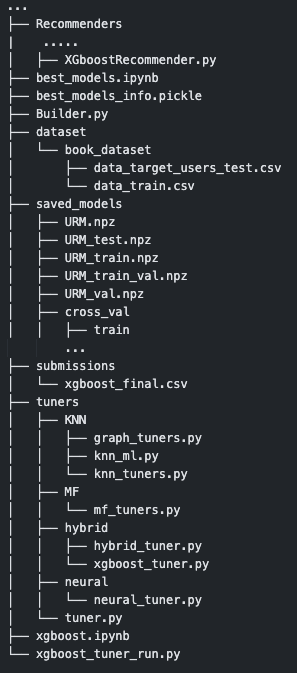
\includegraphics[width=0.25\textwidth]{tree_structure.png}
      \caption{Directory tree structure}
  \end{figure}
\end{frame}

\begin{frame}{Recommendation Algorithms Comparison}
  \begin{columns}[t]
    \begin{column}{0.5\textwidth}
      \textbf{KNN Collaborative Filtering}
      \begin{itemize}
        \item Item-Based
        \begin{itemize}
          \item BM-25
          \item $\text{MAP@}10=0.03493$
        \end{itemize}
        \item User-Based
        \begin{itemize}
          \item TF-IDF
          \item $\text{MAP@}10=0.03493$
        \end{itemize}
      \end{itemize}
    \end{column}
    
    \begin{column}{0.5\textwidth}
      \textbf{Graph-based}
      \begin{itemize}
        \item P3alpha
        \begin{itemize}
            \item $k=40$
            \item $\text{MAP@}10=0.04793$
        \end{itemize}
        \item RP3beta
        \begin{itemize}
          \item $k=28$
          \item $\text{MAP@}10=0.04899$
        \end{itemize}
      \end{itemize}
    \end{column}
  \end{columns}
\end{frame}

\begin{frame}{Recommendation Algorithms Comparison}
  \begin{columns}[t]
    \begin{column}{0.5\textwidth}
      \textbf{Matrix Factorization}
      \begin{itemize}
        \item IALS
        \begin{itemize}
          \item $k=80$ latent factors
          \item $\text{MAP@}10=0.03230$
        \end{itemize}
      \end{itemize}
      \textbf{Neural}
      \begin{itemize}
        \item MultVAERecommender
        \begin{itemize}
          \item $\text{MAP@}10=0.037868$
        \end{itemize}
      \end{itemize}
    \end{column}
    
    \begin{column}{0.5\textwidth}
      \textbf{Item-Based CF}
      \begin{itemize}
        \item SLIMElasticNet
        \begin{itemize}
            \item $k=570$
            \item $\text{MAP@}10=0.05003$
        \end{itemize}
        \item SLIMBRP
        \begin{itemize}
            \item $\text{MAP@}10=0.03893$
        \end{itemize}
      \end{itemize}
    \end{column}
  \end{columns}
\end{frame}


\begin{frame}{Hybrid Models}
  \textbf{ScoresHybrid}
  \begin{itemize}
    \item \texttt{SLIMElasticNet}, \texttt{RP3beta}
    \item $\alpha=0.50282$
    \item $\text{MAP@}10=0.05104$
  \end{itemize}
  \vspace{1cm}
  \begin{center}
    $\tilde{R} = \alpha \cdot \tilde{R_{A}} + (1-\alpha) \cdot \tilde{R_{B}}$
  \end{center}
\end{frame}


\begin{frame}{XGBoost (Preprocessing)}
  \begin{itemize}
    \item Candidate generation selection
    \item Candidate generation cut-off selection
    \item Feature engineering
    \item Categorical features encoding
  \end{itemize}
\end{frame}


\begin{frame}{XGBoost (Candidate Generation)}
  \begin{columns}[t]
    \begin{column}{0.5\textwidth}
      \begin{itemize}
        \item \textbf{ScoresHybrid}
        \begin{itemize}
          \item \texttt{SLIMElasticNet}, \texttt{RP3beta}
          \item Metric: \texttt{Recall}
          \item $\text{Cut-off}=35$
          \item $\alpha=0.36771$
          \item $\text{RECALL@}35=0.24885$
        \end{itemize}
      \end{itemize}
    \end{column}

    \begin{column}{0.5\textwidth}
      \begin{itemize}
        \item \texttt{SLIMElasticNet}
        \begin{itemize}
          \item Metric: \texttt{Recall}
          \item $\text{Cut-off}=35$
          \item $\text{RECALL@}35=0.24221$
        \end{itemize}
        \item \texttt{RP3beta}
        \begin{itemize}
          \item Metric: \texttt{Recall}
          \item $\text{Cut-off}=35$
          \item $\text{RECALL@}35=0.24156$
        \end{itemize}
      \end{itemize}
    \end{column}
  \end{columns}
\end{frame}


\begin{frame}{XGBoost (Feature Engineering)}
  \begin{columns}[t]
    \begin{column}{0.5\textwidth}
      \begin{itemize}
        \item Chosen scores:
        \begin{itemize}
          \item \texttt{SLIMElasticNet}
          \item \texttt{RP3beta}
          \item \texttt{ItemKNNCF}
          \item \texttt{TopPopular}
          \item \texttt{IALS}
          \item \texttt{MultVAE}
        \end{itemize}
        \item Metric: \texttt{NDCG}
        \item $\text{Cut-off}=10$
      \end{itemize}
    \end{column}

    \begin{column}{0.5\textwidth}
      \begin{itemize}
        \item \lstinline{k=[3, 10, 20]}
        \begin{itemize}
          \item \texttt{is\_in\_top\_k()}
          \item \texttt{count\_agreement()}
        \end{itemize}
        \item \texttt{score\_stats()}
        \begin{itemize}
          \item \texttt{mean}
          \item \ldots
          \item \texttt{iqr}
        \end{itemize}
        \item \texttt{normalize\_scores()}
        \item \texttt{disagreement()}
        \item $n_{groups}=20$
        \begin{itemize}
          \item \texttt{user\_profile()}
          \item \texttt{item\_profile()}
          \item $\text{MAP@}10=0.051485$
        \end{itemize}
      \end{itemize}
    \end{column}
  \end{columns}
\end{frame}


\begin{frame}{XGBoost (Categorical Features)}
  \begin{itemize}
    \item naive $\texttt{enable\_categorical}=True$ (Used approach)
    \item Truncated SVD ($k=100 \approx$ 10\% explained variance)
    \item What I did not tried:
    \begin{itemize}
      \item Target encoding
      \item Matrix Factorization
      \item One-hot encoding
      \item Embeddings
    \end{itemize}
  \end{itemize}
\end{frame}


% Conclusion slide
\section{Conclusion}

\begin{frame}{Conclusion}
\begin{itemize}
    \item Thank you for your attention!
    \item Feel free to check out the project on GitHub: \\
    \faGithub\ \url{https://github.com/lorecampa/RecSysChallenge2023}
\end{itemize}
\end{frame}

\end{document}
